\chapter{Experimental results with spatio-angular microscope}
\label{sec:results}

einer der ersten versuche akzeptanzwinkel in abhaengigkeit vom immersionsmedium

dafuer zeigt der focal plane slm einen moeglichst grossen kreis an und
ein kleines fenster wird ueber die pupille bewegt 

fuer jeden punkt auf der pupille wird das gesamte von der kamera
detektierte licht summiert und in ein bild eingetragen

auf diesem bild sieht man indirekt den akzeptanzwinkel, denn wenn man
ueber den hinausgeht, dann wird das anregungslicht totalreflektiert
und fluoreszenslicht bleibt weg

hier wurde das mit drei einfach herzustellenden sampeln erzeugt

duenne schicht fluoreszenter marker pen wurde auf drei slides aufgebracht



\begin{figure}[H]
  \centering
  %\input{tirf-exp.eps_tex} 
  \svginput{1}{tirf-exp}
%  \includegraphics[height=40mm]{screen_mma-disk-integrate_rot}
  \caption{A fluorescent plane on a slide is embedded in oil, water or
    air. The thickness of the embedding medium is approximately
    $\unit[5]{\mu m}$. The focal plane SLM illuminates a disk with $\unit[30]{\mu
      m}$ diameter while a $15\times 15$ window is scanned over the
    MMA. The window corresponds to a square with $\unit[210]{\mu m}$
    on the side as opposed to \unit[3.6]{mm} BFP diameter {\bf right top:} 
    Typical camera image, the orange circle indicates the $\unit[30]{\mu
      m}$ illuminated area.
% 200 px diameter on LCoS
% 15x15 px full diameter is D=2*(R=f*NA) f=164.5/63=2.61  NA=1.38
% D=3.6mm -> D/256*15 = 210 um
    camera image.}
  \label{fig:tirf-exp}
\end{figure}





gel with fluorophore \cite{Ruckerl}
\begin{figure}[!hbt]
  \centering
  \svginput{1}{overview-bleach}
  \caption{The confocal measurements and images were kindly provided
    by Florian R\"uckerl (Institut Pasteur).}
  \label{fig:overview-bleach}
\end{figure}

\comment{
\jpginput{}{m_wf}{}
}

\begin{figure}[H]
  \centering
  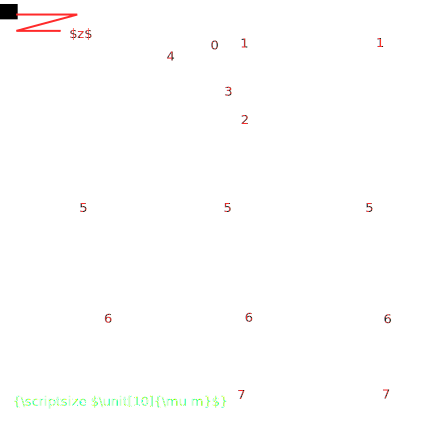
\includegraphics[width=12cm]{m_wf}
  \caption{Wide field stack of a three-dimensional distribution of
    yellow-green beads in agar. Sampling in $z$ is $\unit[1]{\mu m}$.}
  \label{fig:m_wf}
\end{figure}


\begin{figure}[H]
  \centering
  \svginput{1}{m_sec}
  \caption{Computationally sectioned images. Note that two beads (4
    and 7) are very close to the border of the field of view and not
    fully illuminated.}
  \label{fig:m_sec}
\end{figure}


\begin{figure}[H]
  \centering
  \svginput{1}{angular-beads}
  \caption{Spatio-angular controlled illumination of the beads from
    \figref{fig:m_sec}. The top left image shows bead number zero and
    so forth, the second image in the top shows bead number one and so
    on. The LCoS selectively illuminates the target bead and the MMA
    displays the pattern shown in \figref{fig:m_bfp_co}.}
  \label{fig:m_ang}
\end{figure}


\begin{figure}[!hbt]
  \centering
  \svginput{1}{montage-ang}
  \caption{}
  \label{fig:montage-ang}
\end{figure}




%%% Local Variables: 
%%% mode: latex
%%% TeX-master: "kielhorn_memi"
%%% End: 
